\section{繁花规}
\markboth{42. 繁花规}{42. 繁花规}

从百货公司可以买到一种价廉物美的儿童玩具，叫做繁花规。繁花规由一套彩色塑料齿轮组成。一个大齿轮是环状的，牙齿做在里面；几个小齿轮的牙齿做在外面，小齿轮内部有一些小圆洞和几个其他形状的较大的洞。玩的时候，用左手按住大齿轮，让它紧贴在纸上，不能移动，在大齿轮里放一只小齿轮，如图 42.1(1) 所示，把笔尖插进小齿轮的某一个洞里，让小齿轮紧贴大齿轮内壁滚动，笔尖就会在纸上画出美丽的曲线花纹。利用不同的小齿轮和小齿轮上不同的洞，可以画出很多不同形状的复杂精巧的花纹。图 42.1(2) $\sim$ (5) 就是用繁花规画出的几幅花纹图案，它们都是变幅内摆线，不过为了美观，有几幅图中的变幅内摆线只画了一部分。

\begin{figure}[htbp]
  \centering
  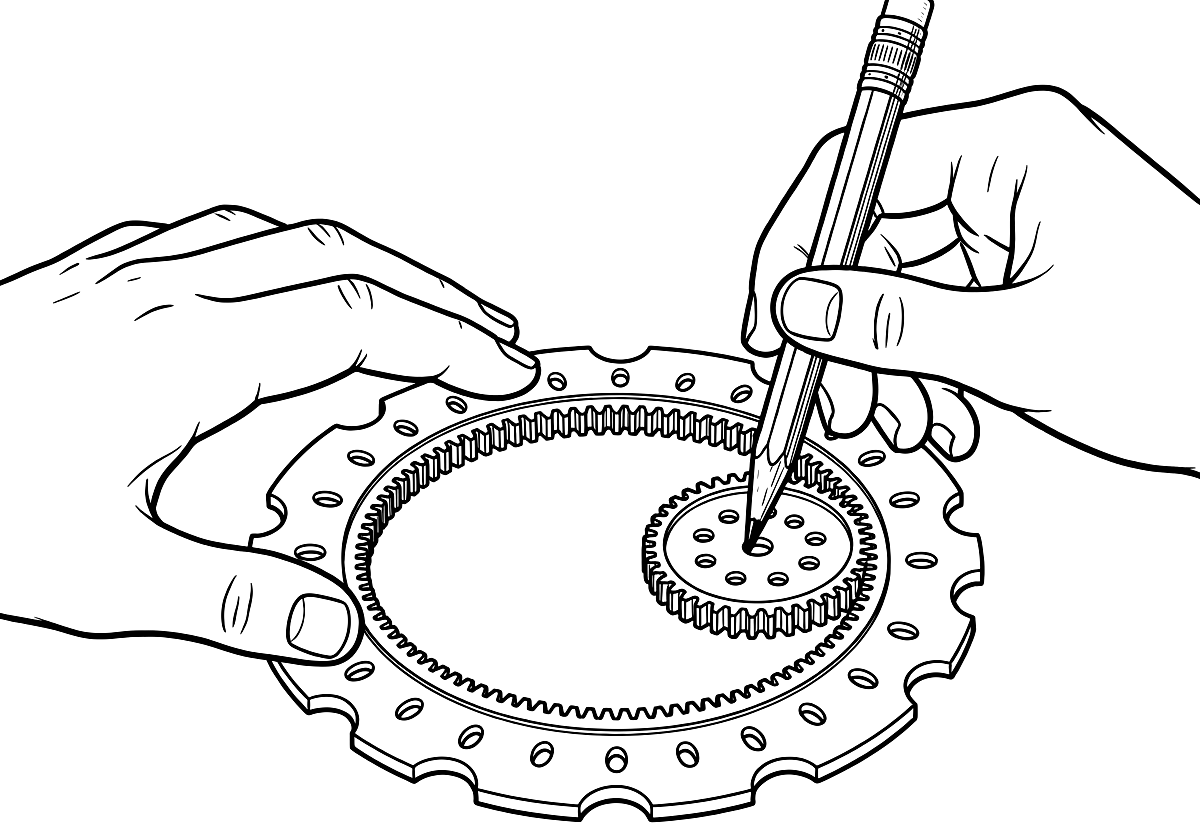
\includegraphics[width=0.48\textwidth]{fig_042_1.png}
  \par\vspace{2pt}
  {\footnotesize (1)}

  \vspace{6pt}
  \begin{minipage}[b]{0.48\textwidth}
    \centering
    \begin{tikzpicture}[scale=1.48, line cap=round, line join=round]
      % (2) 18 瓣四层套叠繁花规花环 (m = 5/18, 1-m = 13/18, k = 13/5 = 2.6)
      \def\om{0.722222}
      \def\kval{2.6}
      \foreach \h/\ph in {0.56/0, 0.51/3, 0.46/6, 0.41/9} {
        \foreach \n in {0,1,2,3,4} {
          \pgfmathsetmacro{\ta}{360*\n}
          \pgfmathsetmacro{\tb}{360*(\n+1)}
          \draw[line width=0.55pt, curveblue!90!black, domain=\ta:\tb, samples=72, variable=\t]
            plot ({\om*cos(\t)+\h*cos(\kval*\t+\ph)},
                  {\om*sin(\t)-\h*sin(\kval*\t+\ph)});
        }
      }
    \end{tikzpicture}
    \par\vspace{2pt}{\footnotesize (2)}
  \end{minipage}
  \hfill
  \begin{minipage}[b]{0.48\textwidth}
    \centering
    \begin{tikzpicture}[scale=1.51, line cap=round, line join=round]
      % (3) 32 瓣细密放射菊花纹 (m = 11/32, 1-m = 21/32, k = 21/11)
      \def\om{0.65625}
      \def\kval{1.9090909}
      \def\h{0.60}
      \foreach \n in {0,1,...,10} {
        \pgfmathsetmacro{\ta}{360*\n}
        \pgfmathsetmacro{\tb}{360*(\n+1)}
        \draw[line width=0.58pt, curveblue!90!black, domain=\ta:\tb, samples=72, variable=\t]
          plot ({\om*cos(\t)+\h*cos(\kval*\t)},
                {\om*sin(\t)-\h*sin(\kval*\t)});
      }
    \end{tikzpicture}
    \par\vspace{2pt}{\footnotesize (3)}
  \end{minipage}

  \vspace{6pt}
  \begin{minipage}[b]{0.48\textwidth}
    \centering
    \begin{tikzpicture}[scale=3.03, line cap=round, line join=round]
      % (4) 28 瓣圆浑菱形编织网球 (m = 19/28, 1-m = 9/28, k = 9/19)
      \def\om{0.3214286}
      \def\kval{0.4736842}
      \def\h{0.305}
      \foreach \n in {0,1,...,18} {
        \pgfmathsetmacro{\ta}{360*\n}
        \pgfmathsetmacro{\tb}{360*(\n+1)}
        \draw[line width=0.58pt, curveblue!90!black, domain=\ta:\tb, samples=56, variable=\t]
          plot ({\om*cos(\t)+\h*cos(\kval*\t)},
                {\om*sin(\t)-\h*sin(\kval*\t)});
      }
    \end{tikzpicture}
    \par\vspace{2pt}{\footnotesize (4)}
  \end{minipage}
  \hfill
  \begin{minipage}[b]{0.48\textwidth}
    \centering
    \begin{tikzpicture}[scale=1.45, line cap=round, line join=round]
      % (5) 3 叶旋转丝带非闭合变幅内摆线 (m = 21/64, 1-m = 43/64, k = 43/21, 绘制 11 圈)
      \def\om{0.671875}
      \def\kval{2.047619}
      \def\h{0.64}
      \foreach \n in {0,1,...,10} {
        \pgfmathsetmacro{\ta}{360*\n}
        \pgfmathsetmacro{\tb}{360*(\n+1)}
        \draw[line width=0.58pt, curveblue!90!black, domain=\ta:\tb, samples=72, variable=\t]
          plot ({\om*cos(\t)+\h*cos(\kval*\t+18)},
                {\om*sin(\t)-\h*sin(\kval*\t+18)});
      }
    \end{tikzpicture}
    \par\vspace{2pt}{\footnotesize (5)}
  \end{minipage}
  \caption*{图\ 42.1}
\end{figure}
